\documentclass[11pt]{amsart}          
\usepackage[a4paper,verbose]{geometry}
\geometry{top=3cm,bottom=3cm,left=3cm,right=3cm,textheight=595pt}
\setlength{\parskip}{0.3em}
% ==============================
% PACKAGES
% ==============================

\usepackage{amsfonts}
\usepackage{amssymb}  
\usepackage{amsthm} 
\usepackage{amsmath} 
\usepackage{caption}
\usepackage[inline]{enumitem}
\setlist{itemsep=0em, topsep=0em, parsep=0em}
\setlist[enumerate]{label=(\alph*)}
\usepackage{etoolbox}
\usepackage{stmaryrd} 
\usepackage[dvipsnames]{xcolor}
\usepackage[]{hyperref}
\hypersetup{
  colorlinks,
  linkcolor=blue,
  citecolor=blue,
  urlcolor=blue}
\usepackage{graphicx}
\graphicspath{{assets/}}
\usepackage{mathtools}

\usepackage{tikz-cd}
\usepackage{minted}
\usepackage{float}
\usetikzlibrary{
  matrix,
  arrows,
  shapes
}

\setcounter{tocdepth}{1} % Sets depth for table of contents. 

% ======================================
% MACROS
%
% Add your own macros below here
% ======================================

\newcommand{\rr}{{\mathbb{R}}}
\newcommand{\nn}{{\mathbb{N}}}
\newcommand{\iso}{\cong}
\newcommand{\too}{\longrightarrow}
\newcommand{\tto}{\rightrightarrows}
\newcommand{\To}[1]{\xrightarrow{#1}}
\newcommand{\Too}[1]{\To{\;\;#1\;\;}}
\newcommand{\from}{\leftarrow}
\newcommand{\From}[1]{\xleftarrow{#1}}
\newcommand{\Cat}[1]{\mathbf{#1}}
\newcommand{\cat}[1]{\mathcal{#1}}
\newtheorem*{remark}{Remark}
\renewcommand{\ss}{\subseteq}
\newcommand{\hask}[1]{\mintinline{Haskell}{#1}}
\newenvironment{haskell}
  {\VerbatimEnvironment
  	\begin{minted}[escapeinside=??, mathescape=true,frame=single, framesep=5pt, tabsize=1]{Haskell}}
  {\end{minted}}

% ======================================
% FRONT MATTER
% ======================================

\author{Bartosz Milewski}
\title{Fixed Points of Endofunctors}

\begin{document}
\section{Expressions}
When we see an algebraic expression like
\[x^2 + 2 x + 3\]
we parse it as a tree. We start with

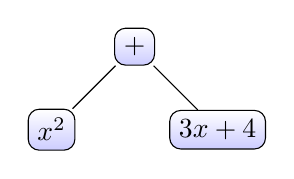
\begin{tikzpicture}[
    level distance=3em,
  every node/.style = {shape=rectangle, rounded corners,
    draw, align=center,
    top color=white, bottom color=blue!20}]
    \tikzstyle{level 1}=[sibling distance=6em]
  \node {$+$}
    child { node {$x^2$} }
    child { node {$3 x + 4$} };
\end{tikzpicture}

We then recursive expand the nodes

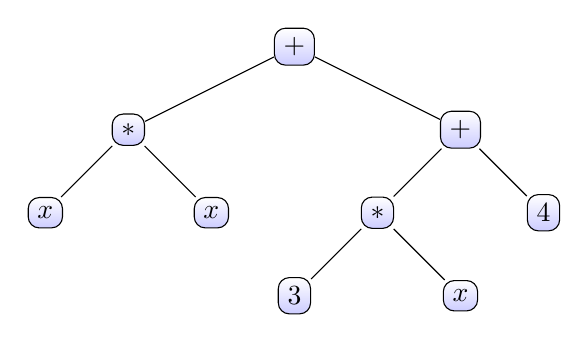
\begin{tikzpicture}[
    level distance=3em,
  every node/.style = {shape=rectangle, rounded corners,
    draw, align=center,
    top color=white, bottom color=blue!20}]
    \tikzstyle{level 1}=[sibling distance=12em]
    \tikzstyle{level 2}=[sibling distance=6em]
  \node {$+$}
    child { node {$*$} 
       child { node {$x$} } 
       child { node {$x$} } }
    child { node {$+$}
      child { node {$*$}
        child { node {$3$} }
        child { node {$x$} } }
      child { node {$4$} } };
\end{tikzpicture}

A parser of algebraic expressions would parse it into a tree data structure

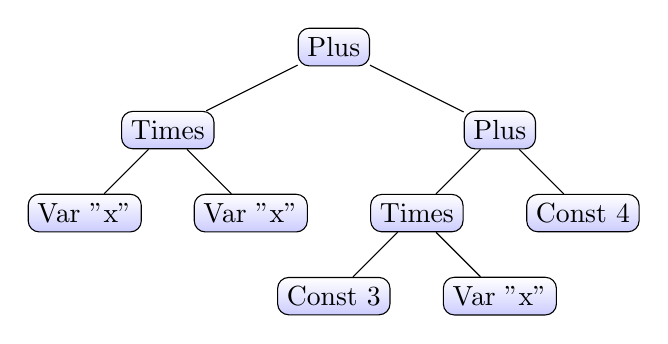
\begin{tikzpicture}[
    level distance=3em,
  every node/.style = {shape=rectangle, rounded corners,
    draw, align=center,
    top color=white, bottom color=blue!20}]
    \tikzstyle{level 1}=[sibling distance=12em]
    \tikzstyle{level 2}=[sibling distance=6em]
  \node {Plus}
    child { node {Times} 
       child { node {Var "x"} } 
       child { node {Var "x"} } }
    child { node {Plus}
      child { node {Times}
        child { node {Const 3} }
        child { node {Var "x"} } }
      child { node {Const 4} } };
\end{tikzpicture}

\section{Examples}
\begin{haskell}
data F a = Leaf 
         | Node a a
  deriving Show
\end{haskell}
\[F a = 1 + a^2\]

\begin{haskell}
instance Functor F where
  fmap _ Leaf       = Leaf
  fmap f (Node x y) = Node (f x) (f y)
\end{haskell}
Let's consider, for instance, terms of type \hask{F Int}. It's either a \hask{Leaf} or a \hask{Node} with two numbers in it
\begin{haskell}
x1, y1 :: F Int
x1 = Leaf
y1 = Node 1 2
\end{haskell}
Here are some values of the type \hask{F (F Int)}
\begin{haskell}
x2, y2 :: F (F Int)
x2 = Leaf
y2 = Node x1 y1
\end{haskell}
We can display \hask{y2}
\begin{haskell}
> Node Leaf (Node 1 2)
\end{haskell}
Lifting a function $f \colon a \to b$ to $F^2$ can be described as applying \hask{fmap} twice. Here's the action of \hask{(+1)} on our test values
\begin{haskell}
fmap (fmap (+1)) x2
> Leaf
fmap (fmap (+1)) y2
> Node Leaf (Node 2 3)
\end{haskell}
You can see that \hask{Leaf}s at any level remain untouched; only the contents of bottom \hask{Node}s in the tree are transformed.

\subsection{Initial algebra as a colimit}

Now let's apply powers of $F$ to the initial object, which we define as
\begin{haskell}
data Void
  deriving Show
\end{haskell}
The \hask{Show} instance for \hask{Void} requires the pragma
\begin{haskell}
{-# language EmptyDataDeriving #-}
\end{haskell}
Even though there are no values of the type \hask{Void}, we can still constructy a value of the type \hask{F Void}
\begin{haskell}
z1 :: F Void
z1 = Leaf
\end{haskell}
This is a very important property of our $F$: its action on the empty set does not produce an empty set. This is what allows us to generate a non-trivial sequence of powers of $F$ starting with the empty set. The colimit of this sequence is the initial algebra. 

Au contraire, the same construction for a functor that generates infinite streams
\begin{haskell}
data StreamF a x = ConsF a x
\end{haskell}
will produce an uninhabited initial algebra--which is different from its terminal coalgebra, that is
\begin{haskell}
data Stream a = ConsF a (Stream a)
\end{haskell}

Double application of our \hask{F} to \hask{Void} produces a new \hask{Leaf} and a \hask{Node} that contains two \hask{Leaf}s. Notice the duplication: a \hask{Leaf} is produced at both (in fact, at all non-zero) powers of $F$ acting on \hask{Void}
\begin{haskell}
z2, v2 :: F (F Void)
z2 = Leaf
v2 = Node z1 z1
> Node Leaf Leaf
\end{haskell}
Powers of $F$ acting on \hask{Void} generate trees which terminate with \hask{Leaf}s but no terminal \hask{Node}s. 
Since we are starting with \hask{Void}, the only function that we can apply or lift is
\begin{haskell}
absurd :: Void -> a
absurd a = case a of {}
\end{haskell}
This definition requires another pragma
\begin{haskell}
{-# language EmptyCase #-}
\end{haskell}

Lifting \hask{absurd} doesn't change the shapes of these trees.
\begin{haskell}
z1' :: F (F Void)
z1' = fmap absurd z1
> Leaf
\end{haskell}

\begin{haskell}
z2', v2' :: F (F (F Void))
z2' = fmap (fmap absurd) z2
> Leaf
v2' = fmap (fmap absurd) v2
> Node Leaf Leaf
\end{haskell}

Higher and higher powers of $F$ acting on \hask{Void} will eventually produce any tree. But for any given power, there will exist even larger trees that are not generated by it. 

On the other hand, if we were to take a sum (a coproduct) of all (infinitely many) powers, we'll get all the trees, but also a lot of duplication. For instance, \hask{z1} is the same tree as \hask{z2}, and so on. We have to have a way of identifying multiply generated trees. This is what a \textit{colimit} of a chain of powers will accomplish. 

A colimit in $Set$ is a sum, or a discriminated union, in which we identify all the injections that are connected by morphisms in the cocone base. 

\begin{figure}[H]
\centering
\begin{tikzcd}
  0
  \arrow[r, "!"]
  \arrow[d, ""]
   \arrow[d, "\iota_0"]
   &F 0
   \arrow[r, "F !"]
   \arrow[dl, "\iota_{(F 0)}"]
   &F^2 0
   \arrow[r, dashed]
   \arrow[dll, bend left, "\iota_{(F^2 0)}"]
   & ...
   \\
   \mu F
\end{tikzcd}
\end{figure}

Here we use the lifted \hask{absurd} (or $!$ in the picture above) as the morphisms that connect the powers of $F$ acting of \hask{Void} (or $0$ in the picture). 

In particular, \hask{fmap absurd} maps the leaf generated by \hask{F Void} to the leaf generated by \hask{F (F Void)}, and so on. All trees generated by the $n$'th power of $F$ are injected into the $n+1$'st power of $F$ by \hask{absurd} lifted by the $n$th power of $F$. The colimit is formed by equivalence classes with respect to these identifications. In particular, there is a class for a tree consisting of a single leaf whose representative can be taken from \hask{F Void} or from \hask{F (F Void)} and so on. 

\subsection{Terminal coalgebra as a limit}

Things are different with powers of $F$ acting on the terminal object: singleton or unit type. We get trees with both terminal \hask{Leaf}s and terminal \hask{Node}s that contain units
\begin{haskell}
w1, u1 :: F ()
w1 = Leaf
u1 = Node () ()
\end{haskell}
The square of $F$ produces, among others,
\begin{haskell}
w2, u2, t2, s2 :: F (F ())
w2 = Leaf
> Leaf
u2 = Node w1 w1
> Node Leaf Leaf
t2 = Node w1 u1
> Node Leaf (Node () ())
s2 = Node u1 u1
> Node (Node () ()) (Node () ())
\end{haskell}
This time we are interested in mapping into the terminal object
\begin{haskell}
unit :: a -> ()
unit _ = ()
\end{haskell}
We are going to lift \hask{unit} to transform $F^{n + 1} 1$ to $F^n 1$. 

Applying \hask{unit} directly to \hask{F ()} turns it into \hask{()}. 

Values of the type $F^2 1$ are mapped to values of the type $F 1$
\begin{haskell}
w2' = fmap unit w2
> Leaf
u2' = fmap unit u2
> Node () ()
t2' = fmap unit t2
> Node () ()
s2' = fmap unit s2
> Node () ()
\end{haskell}
and so on.

The following pattern emerges. $F^n 1$ contains trees that end with either leaves or the values of the unit type. The latter play the role of potential seeds. Each seed can give rise to any value of the type \hask{F ()}, be it a leaf or a node. Normally, we use a particular coalgebra to generate these values from a carrier, which serves as the seed. Here, we are modeling a situation where a singleton seed generates the whole set of all possible values. It's a "universal" seed.

Except that we are reversing the process: by lifting \hask{unit} we transform $F^{n+1}$ to $F^n$. Instead of expanding the seeds, we are shrinking single-level trees, or buds, back to their seeds. For instance, take
\begin{haskell}
t2 :: F (F ())
t2 = Node w1 u1
> Node Leaf (Node () ())
\end{haskell}
which has two buds, \hask{Leaf} and \hask{Node () ()}. \hask{fmap unit} shrinks it down to \hask{Node () ()}. We can thing of the ``inverse'' of the lifted \hask{unit} to generate all possible trees of the next level from the universal seeds embedded in the previous level.

Since a terminal coalgebra is dual to intial algebra, we can generate it as a limit of a sequence that contains powers of $F$ acting on \hask{()} connected by lifted \hask{unit}s. A limit in $Set$ is equivalent to a set of cones whose tip is the singleton set. The base of such cone is a sequence of $F^n 1$, starting with $1$. The arrows in the base are lifted \hask{unit}s (or $\mbox{!`}$ in the picture below) pointing from $F^{n + 1} 1$ to $F^n 1$. 

\begin{figure}[H]
\centering
\begin{tikzcd}
  1
  \arrow[d, "\pi_1"]
  \arrow[dr, "\pi_{(F 1)}"]
  \arrow[drr, bend left, "\pi_{(F^2 1)}"]
  \\
  1
  & F 1
  \arrow[l, "\mbox{!`}"]
  & F^2 1
  \arrow[l, "F \mbox{!`}"]
  & ...
  \arrow[l, dashed]
\end{tikzcd}
\end{figure}
This chain is infinite, so it's not immediately obvious what part of the cone is relevant. But imagine that the chain terminates on the right. Then the rightmost projection uniquely determines all the others (all the triangles commute). 

Notice also that if we select a leaf-terminated tree, such as \hask{Node Leaf Leaf}, than all the values to the right of it (with higher powers of $F$) in the sequence must all be the same. For instance, the third power of $F$ 
\begin{haskell}
w3 :: F (F (F ()))
w3 = Node Leaf Leaf
\end{haskell}
is mapped to the second power of $F$ that gives the same tree
\begin{haskell}
w3' :: F (F ())
w3' = fmap (fmap unit) w3
> Node Leaf Leaf
\end{haskell}
This way, all finite trees are generated from cones that eventually reach a stable point on the right. However, there are cones that never stabilize, and those correspond to infinite trees. 

The \hask{StreamF} functor, in particular, doesn't produce leaves, so all its cones are infinite, corresponding to infinite \hask{Stream}s.

\section{Adjunction}
There is an obvious forgetful functor $U$ from the category of $F$-algebras to $Set$. Under certain conditions, the left adjoint free functor $\Phi$ exists
\[C^F ( \Phi x, a) \cong C(x, U a)\]
This adjunction can be evaluated at the initial object---the empty set. 
\[C^F ( \Phi 0, a) \cong C(0, U a)\]
This shows that there is a unique algebra morphism---the catamorphism--- from $\Phi 0$ to any algebra $a$.

Conversely, there is a cofree functor $\Psi$
\[C_F(c, \Psi x) \cong C(U c, x)\]
It can be evaluated at a terminal object
\[C_F(c, \Psi 1) \cong C(U c, 1)\]
showing that there is a unique coalgebra morphism---the anamorphism---from any coalgebra $c$ to $\Psi 1$.


\section{Fixed point}

In Haskell, the least fixed point and the greatest fixed point, are often given by the same formula
\begin{haskell}
newtype Fix f = Fix { unFix :: f (Fix f) }
\end{haskell}

We can still define them separately by directly encoding their universal property. 

\section{Initial algebra and catamorphism}

The initial algebra can be defined by its mapping out property.

\begin{haskell}
newtype Mu f = Mu (forall a. (f a -> a) -> a)
\end{haskell}
Notice that this definition requires the following language pragma
\begin{haskell}
{-# language RankNTypes #-}
\end{haskell}
This definition works because for every least fixed point one can define a catamorphism, which can be rewritten as
\begin{haskell}
cata :: Functor f => Fix f -> (forall a . (f a -> a) -> a)
cata (Fix x) = \alg -> alg (fmap (flip cata alg) x)
\end{haskell}
(\hask{flip} is a function that reverses the order of arguments of its (function) argument.) What the definition of \hask{Mu} is saying is that it's an object that, for all algebras, has a mapping out to a catamorphism.

It's easy to define a catamorphism in terms of \hask{Mu}, since \hask{Mu} \emph{is} a catamorphism
\begin{haskell}
cataMu :: Functor f => Algebra f a -> Mu f -> a
cataMu alg (Mu cata) = cata alg
\end{haskell}
The challenge is to construct terms of type \hask{Mu f}. For instance, let's convert a list of \hask{a} to a term of type \hask{Mu (ListF a)}
\begin{haskell}
mkList :: forall a. [a] -> Mu (ListF a)
mkList as = Mu cata
  where cata :: forall x. (ListF a x -> x) -> x
        cata unf = go as
          where
            go [] = unf NilF
            go (n: ns) = unf (ConsF n (go ns))
\end{haskell}
Notice that we use the type \hask{a} defined in the type signature of \hask{mkList} to define the type signature of the helper function \hask{cata}. For the compiler to identify the two, we have to use the pragma
\begin{haskell}
{-# language ScopedTypeVariables #-}
\end{haskell}
You can now verify that
\begin{haskell}
cataMu sumAlg (mkList [1..10])
\end{haskell}
produces the correct result for the following algebra
\begin{haskell}
sumAlg :: Algebra (ListF Int) Int
sumAlg NilF = 0
sumAlg (ConsF a x) = a + x
\end{haskell}

\section{Terminal coalgebra and anamorphism}

The terminal coalgebra, on the other hand, is defined by its mapping in property. This requires a definition in terms of existential types. If Haskell had an existential quantifier, we could write the following definition for the terminal coalgebra
\begin{haskell}
data Nu f =  Nu (exists a. (a -> f a, a))
\end{haskell}
Existential types can be encoded in Haskell using the so called Generalized Algebraic Data Types or GADTs
\begin{haskell}
data Nu f where 
  Nu :: (a -> f a) -> a -> Nu f
\end{haskell}
The use of GADTs requires the language pragma 
\begin{haskell}
{-# language GADTs #-}
\end{haskell}

The argument is that, for every greatest fixed point one can define an anamorphism

\begin{haskell}
ana :: Functor f => forall a. (a -> f a) -> a -> Fix f
ana coa x = Fix (fmap (ana coa) (coa x))
\end{haskell}
We can uncurry it
\begin{haskell}
ana :: Functor f => forall a. (a -> f a, a) -> Fix f
ana (coa, x) = Fix (fmap (curry ana coa) (coa x))
\end{haskell}
A universally quantified mapping out 
\begin{haskell}
forall a. ((a -> f a, a) -> Fix f)
\end{haskell}
is equivalent to a mapping out of an existential type (in pseudo-Haskell)
\begin{haskell}
(exists a. (a -> f a, a)) -> Fix f
\end{haskell}
which is the type signature of the constructor of \hask{Nu f}.

The intuition is that, if you want to implement a function from an existential type---a type which hides some other type \hask{a} to which you have no access---your function has to be prepared to handle any \hask{a}. In other words, it has to be polymorphic in \hask{a}. 

Since in an existential type we have no access to the hidden type, it has to provide both the ``producer'' and the ``consumer'' for this type. Here we are given a value of type \hask{a} on the produces side, and the function \hask{a -> f a} as the consumer. All we can do is to apply this function to \hask{a} and obtain the term of the type \hask{f a}. Since \hask{f} is a functor, we can lift our function and apply it again, to get something of the type \hask{f (f a)}. Continuing this process, we can obtain arbitrary powers of \hask{f} acting on \hask{a}. We get a recursive data type.

An anamorphism in terms of \hask{Nu} is given by
\begin{haskell}
anaNu :: Functor f => Coalgebra f a -> a -> Nu f
anaNu coa a = Nu coa a
\end{haskell}

Notice however that we cannot directly pass the result of \hask{anaNu} to \hask{cataMu} because we are no longer guaranteed that the initial algebra is the same as the terminal coalgebra for a given functor.

\section{End/Coend formulation}

Let's rewrite \hask{Mu} using GADTs
\begin{haskell}
data Mu f where
  Mu :: (forall a. (f a -> a) -> a) -> Mu f
\end{haskell}
We use a natural transformation to construct a \hask{Mu}. Categorically, we can write it as an end
\[\mu f = \int_a a^{C(f a, a)}\]
It's an end over the profunctor
\[p a b = b^{ C(f b, a)}\]
Where the power is defined as
\[ C(x, a^s) \cong Set(s, C(x, a)) \]

Projection from the end is a catamorphism
\[\pi_a \colon \mu f \to a^{C(f a, a)}\]
It's a morphism from the hom-set
\[C(\mu f, a^{C(f a, a)})\]
or an element of
\[Set(C(f a, a), C(\mu f, a))\]

Similarly, we can rewrite \hask{Nu}
\begin{haskell}
data Nu f where 
  Nu :: (a -> f a) -> a -> Nu f
\end{haskell}
as a coend
\[\nu f = \int^a C(a, f a) \cdot a \]
over the profunctor
\[p a b = C(a, f b) \cdot b\]
where the copower is defined as
\[ C(s \cdot a, x) \cong Set(s, C(a, x))\]

Injection into the coend is an anamorphism
\[ \iota_a \colon C(a, f a) \cdot a \to \nu f\]
It's a morphism from the hom-set
\[C(C(a, f a) \cdot a, \nu f)\]
or an element of
\[Set(C(a, f a), C(a, \nu f))\]

Because of Lambek's lemma, an initial algebra is also a coalgebra, and a terminal coalgebra is also an algebra. Universality, therefore, tells us that there is a unique algebra morphism (as well as a unique coalgebra morphism) 
\[\phi \colon \mu f \to \nu f\]
This is a canonical embedding, but not necessarily an isomorphism.

The two profunctors in the definition of \hask{Mu} and \hask{Nu} can be written as
\begin{haskell}
data M f a b = M ((f b -> a) -> b)
\end{haskell}

\begin{haskell}
instance Functor f => Profunctor (M f) where
  dimap g g' (M h) = M (\j -> g'( h (g . j . fmap g')))
\end{haskell}

\begin{haskell}
data N f a b = N (a -> f b) b
\end{haskell}

\begin{haskell}
instance Functor f => Profunctor (N f) where
  dimap g g' (N h b) = N (fmap g' . h . g) (g' b)
\end{haskell}

\section{Hylomorphism}

If the mapping from from the terminal coalgebra $\nu$ to the initial algebra $\mu$ exists, it is an element of the following hom-set

\[C \Big(\int^a C(a, f a) \cdot a, \int_b b^{C(f b, b)} \Big)\]

By co-continuity of the hom-functor, this is isomorphic to

\[ \int_a C \Big( C(a, f a) \cdot a, \int_b b^{C(f b, b)}\Big)\]

Using continuity we get

\[ \int_{a, b} C \Big( C(a, f a) \cdot a, b^{C(f b, b)}\Big)\]

Using the definition of the copower
\[ C(s \cdot a, x) \cong Set(s, C(a, x))\]
we get
\[ \int_{a, b} Set \Big(C(a, f a), C(a, b^{C(f b, b)})\Big)\]
And using the definition of the power
\[ C(x, a^s) \cong Set(s, C(x, a)) \]
we get
\[ \int_{a, b} Set \Big(C(a, f a), Set\big(C(f b, b), C(a, b)\big)\Big)\]
Finally, applying the currying adjunction we get
\[ \int_{a, b} Set \Big(C(a, f a) \times C(f b, b), C(a, b)\Big)\]
in which you may recognize a hylomorphism

\begin{haskell}
hylo :: Functor f => Coalgebra f a -> Algebra f b -> a -> b
hylo coa alg = alg . fmap (hylo coa alg) . coa
\end{haskell}

\section{Bibliography}
\begin{itemize}
  \item Michael Barr, \href{http://www.math.mcgill.ca/barr/papers/trmclg.pdf}{Terminal coalgebras for endofunctors on sets}
\end{itemize}

\section{Random things}
\subsection{Initial algebra structure map}
\[j \colon f (\mu f) \to \mu f\]
\[C\Big(f (\mu f), \int_b b^{C(f b, b)}\Big)\]
is a member of
\[\int_b C\Big(f (\mu f), b^{C(f b, b)}\Big)\]
Using the definition of the power
\[ C(x, a^s) \cong Set(s, C(x, a)) \]
we get
\[\int_b Set\Big(C(f b, b), C\big( f (\mu f), b\big) \Big)\]
Using Yoneda lemma we replace $b$ with $f (\mu f)$
\[C(f (f (\mu f)), f (\mu f)) \]

\subsection{Terminal coalgebra structure map}
\[k \colon \nu f \to f (\nu f)\]
is a member of
\[ C\Big( \int^a C(a, f a) \cdot a, f  (\nu f) \Big)\]
\[ \int_a C\Big( C(a, f a) \cdot a, f  (\nu f) \Big)\]
Using the definition of the copower
\[ C(s \cdot a, x) \cong Set(s, C(a, x))\]
we get
\[ \int_a Set\Big( C(a, f a), C\big( a, f  (\nu f) \big) \Big)\]
Yoneda lemma
\[ C(f(\nu f), f ( f (\nu f))) \]

\subsection{Kan extensions}
\[\mu f = \int_a a^{C(f a, a)}\]
\[\nu f = \int^a C(a, f a) \cdot a \]
These formulas are reminiscent of Kan extensions. 
For comparison, the right  Kan extension of $g$ along $f$ is given by
\[(Ran_f g) c = \int_a (g a)^{C(c, f a)}\]
The left Kan extension is
\[(Lan_f g) c = \int^a C(f a, c) \cdot g a \]
If $f$ has left and right adjoints, they are given by
\[Ran_f Id \dashv f \dashv Lan_f Id\]
In particular, using the adjunction
\[(Lan_f Id) c = \int^a C(a, (Lan_f Id) c) \cdot a\]
This shows that $(Lan_f Id) c$ is a fixed point of the functor
\[ \Phi(x) = \int^a C(a, x) \cdot a \]

\subsection{Ends as limits}

Twisted arrow category on $\textit{Tw}(\Cat C)$ has, as objects, morphisms in $\Cat C$ (or, strictly speaking, triples $(a, b, f \colon a \to b)$). A morphism from $f \colon a \to b$ to $g \colon a' \to b'$ is a pair of morphisms 
\[(h \colon a' \to a, h' \colon b \to b')\]
For every profunctor $p \colon C^{op} \times C \to \Cat{Set}$ define a functor $\bar p \colon \textit{Tw}(\Cat C) \to Set$. On objects
\[\bar p (a, b, f) = p a b\]
and on morphisms, it's just profunctor lifting.

It can be shown that the end is just a limit over the twisted arrow category
\[\int_c p c c \cong \lim_{Tw(C)} \bar p\]
Similarly, the coend is a colimit over $Tw(C^{op} )^{op}$
\[\int^c p c c \cong \underset {Tw(C^{op})^{op}}  { \mbox{colim}} \bar p\]

\subsection{Iterative solution}
Terminal coalgebra is a limit, and initial algebra is a colimit of these two chains
\begin{figure}[H]
\centering
\begin{tikzcd}
  f (\nu f)
  \\
  \nu f
  \arrow[u, "k"]
  \arrow[d, "\pi_1"]
  \arrow[dr, "\pi_{(f 1)}"]
  \arrow[drr, bend left, "\pi_{(f^2 1)}"]
  \\
  1
  & f 1
  \arrow[l, "\mbox{!`}"]
  & f^2 1
  \arrow[l, "f \mbox{!`}"]
  & ...
  \arrow[l, dashed]
   \\
  0
   \arrow[u, "!"]
  \arrow[r, "!"]
  \arrow[d, ""]
   \arrow[d, "\iota_0"]
   &f 0
   \arrow[u, "f !"]
   \arrow[r, "f !"]
   \arrow[dl, "\iota_{(f 0)}"]
   &f^2 0
   \arrow[u, "f^2 !"]
   \arrow[r, dashed]
   \arrow[dll, bend left, "\iota_{(f^2 0)}"]
   & ...
   \\
   \mu f
   \arrow[uuu, bend left, "\varphi"]
   \\ 
   f (\mu f)
   \arrow[u, "j"]
\end{tikzcd}
\end{figure}

\section{Algebra morphisms}

\begin{tikzcd}
  F[A] 
  \arrow[r,"F(f)"] 
  \arrow[d,"a"'] 
  & F[B] 
  \arrow[d,"b"]
  \\
  A 
  \arrow[r,"f"'] 
  & B
\end{tikzcd}

Composition

\begin{tikzcd}
  F[A] 
  \arrow[r,"F(f)"] 
  \arrow[d,"a"'] 
  & F[B] 
  \arrow[r,"F(g)"]
  \arrow[d,"b"]
  & F[C]
  \arrow[d, "c"]
  \\
  A 
  \arrow[r,"f"'] 
  & B
  \arrow[r, "g"']
  & C
\end{tikzcd}

Identity

\begin{tikzcd}
  F[A] 
  \arrow[r,"id"] 
  \arrow[d,"a"'] 
  & F[A] 
  \arrow[d,"a"]
  \\
  A 
  \arrow[r,"id"'] 
  & A
\end{tikzcd}

Initial algebra

\begin{tikzcd}
  F[I] 
  \arrow[r,"F(m)"] 
  \arrow[d,"j"'] 
  & F[A] 
  \arrow[d,"a"]
  \\
  I 
  \arrow[r,"m"'] 
  & A
\end{tikzcd}

\begin{tikzcd}
  F[Fix[F]] 
  \arrow[r,"F(m)"] 
  \arrow[d, dashed, bend right, "in"'] 
  & F[A] 
  \arrow[d,"alg"]
  \\
  Fix[F]
  \arrow[u, bend right, "out"']
  \arrow[r,"m"'] 
  & A
\end{tikzcd}

\begin{tikzcd}
  F I 
  \arrow[r,"F m "] 
  \arrow[d,"j"'] 
  & F A 
  \arrow[d,"a"]
  \\
  I 
  \arrow[r,"m"'] 
  & A
\end{tikzcd}

\begin{tikzcd}
  F I 
  \arrow[r,"F m "] 
  \arrow[d,"j"'] 
  & F (F I)
  \arrow[d,"F j"]
  \\
  I 
  \arrow[r,"m"'] 
  & F I
\end{tikzcd}


\begin{tikzcd}
  F (F I )
  \arrow[r,"F j "] 
  \arrow[d,"F j"'] 
  & F I
  \arrow[d,"j"]
  \\
  F I 
  \arrow[r,"j"'] 
  & I
\end{tikzcd}


\begin{tikzcd}
  F I 
  \arrow[r,"F m "] 
  \arrow[d,"j"'] 
  & F (F I)
  \arrow[r, "F j"]
  \arrow[d,"F j"]
  & F I
  \arrow[d,"j"]
  \\
  I 
  \arrow[r,"m"'] 
  & F I
  \arrow[r,"j"'] 
  & I
\end{tikzcd}



\end{document}
\maketitle{}